\documentclass{beamer}
\usepackage[utf8]{inputenc}

\usetheme{Madrid}
\usecolortheme{default}
\usepackage{amsmath,amssymb,amsfonts,amsthm}
\usepackage{txfonts}
\usepackage{tkz-euclide}
\usepackage{listings}
\usepackage{adjustbox}
\usepackage{array}
\usepackage{tabularx}
\usepackage{gvv}
\usepackage{lmodern}
\usepackage{circuitikz}
\usepackage{tikz}
\usepackage{graphicx}

\setbeamertemplate{page number in head/foot}[totalframenumber]

\usepackage{tcolorbox}
\tcbuselibrary{minted,breakable,xparse,skins}



\definecolor{bg}{gray}{0.95}
\DeclareTCBListing{mintedbox}{O{}m!O{}}{%
	breakable=true,
	listing engine=minted,
	listing only,
	minted language=#2,
	minted style=default,
	minted options={%
		linenos,
		gobble=0,
		breaklines=true,
		breakafter=,,
		fontsize=\small,
		numbersep=8pt,
		#1},
	boxsep=0pt,
	left skip=0pt,
	right skip=0pt,
	left=25pt,
	right=0pt,
	top=3pt,
	bottom=3pt,
	arc=5pt,
	leftrule=0pt,
	rightrule=0pt,
	bottomrule=2pt,
	toprule=2pt,
	colback=bg,
	colframe=orange!70,
	enhanced,
	overlay={%
		\begin{tcbclipinterior}
			\fill[orange!20!white] (frame.south west) rectangle ([xshift=20pt]frame.north west);
	\end{tcbclipinterior}},
	#3,
}
\lstset{
	language=C,
	basicstyle=\ttfamily\small,
	keywordstyle=\color{blue},
	stringstyle=\color{orange},
	commentstyle=\color{green!60!black},
	numbers=left,
	numberstyle=\tiny\color{gray},
	breaklines=true,
	showstringspaces=false,
}
%------------------------------------------------------------
%This block of code defines the information to appear in the
%Title page
\title %optional
{2.10.75}
%\subtitle{A short story}

\author % (optional)
{RAVULA SHASHANK REDDY - EE25BTECH11047}

 \begin{document}
	
	
	\frame{\titlepage}
	\begin{frame}{Question}
Prove the points with position vectors $\vec{a}+\vec{b},\;\vec{a}-\vec{b}$ and $\vec{a}+k\vec{b}$ are collinear for all real values of   $k$.

\end{frame}
\begin{frame}{Theoretical Solution}
    Given:
\begin{align}
    \vec{P} &= \myvec{\vec{a}&\vec{b}}\myvec{1\\1},\vec{Q}=\myvec{\vec{a}&\vec{b}}\myvec{1\\-1},\vec{R} =\myvec{\vec{a}&\vec{b}}\myvec{1\\k} \\
    \vec{P}-\vec{Q} &=\myvec{\vec{a}&\vec{b}}\myvec{0\\2} \\ 
    \vec{R}-\vec{P} &= \myvec{\vec{a}&\vec{b}}\myvec{0\\k-1}\\[6pt]
    M &= \myvec{ \vec{P}-\vec{Q} & \vec{R}-\vec{P} } 
       = \myvec{ 0 & 0\\2\vec{b} & (k-1)\vec{b} } \\[6pt]
      M& = \vec{b} \myvec{0&0\\2 & k-1}\\
\text{rank}(M) \leq 1.
\end{align}
\begin{center}
Therefore, the two difference vectors are linearly dependent. \\ 
\end{center}
\end{frame}
\begin{frame}{Theoretical Solution}
\begin{center}
Hence, the points $\vec{P}, \vec{Q}, \vec{R}$ are collinear for all real $k$.
\end{center}

For Example:\\ 
\begin{align}
\vec{a}=\myvec{1 \\ 2},\; \vec{b}=\myvec{3 \\ 1}.
\end{align}
For $k=0$:
\begin{align}
\vec{R} = \myvec{1+3(0) \\ 2+0} = \myvec{1 \\ 2}.
\end{align}
For $k=1$:
\begin{align}
\vec{R} = \myvec{1+3(1) \\ 2+1} = \myvec{4 \\ 3}.
\end{align}
For $k=2$:
\begin{align}
\vec{R} = \myvec{1+3(2) \\ 2+2} = \myvec{7 \\ 4}.
\end{align}
\end{frame}
\begin{frame}{Theoretical Solution}

So the three points are:
\begin{align}
\vec{Q} &= \myvec{-2 \\ 1}, 
\vec{P} = \myvec{4 \\ 3}, \\
\vec{R} &= \myvec{1 \\ 2}\;(k=0),\; \myvec{4 \\ 3}\;(k=1),\; \myvec{7 \\ 4}\;(k=2).\\
M(k) &= \myvec{\,\vec{P}-\vec{Q} & \vec{R}-\vec{P}\,} 
     = \myvec{6 & 3k-3 \\[4pt] 2 & k-1}.
\end{align}

For $k=0$:
\begin{align}
M(0) = \myvec{6 & -3 \\ 2 & -1}, \quad \text{rank}(M(0))=1.
\end{align}
\end{frame}
\begin{frame}{Theoretical Solution}

For $k=1$:
\begin{align}
M(1) = \myvec{6 & 0 \\ 2 & 0}, \quad \text{rank}(M(1))=1.
\end{align}

For $k=2$:
\begin{align}
M(2) = \myvec{6 & 3 \\ 2 & 1}, \quad \text{rank}(M(2))=1.
\end{align}

\end{frame}
\begin{frame}[fragile]
    \frametitle{C Code}
    \begin{lstlisting}
        #include <stdio.h>

// Function to compute rank of an n x 2 matrix
// Since columns are multiples, rank is at most 1
int rankMatrix(int n, int col1[], int col2[]) {
    int i;
    // check if both columns are zero
    int zero1 = 1, zero2 = 1;
    for(i=0; i<n; i++) {
        if(col1[i] != 0) zero1 = 0;
        if(col2[i] != 0) zero2 = 0;
    }
    if(zero1 && zero2) return 0; // zero matrix
    // check if col2 is multiple of col1
    int ratio_num = 0, ratio_den = 0;
    \end{lstlisting}
    \end{frame}
\begin{frame}[fragile]
    \frametitle{C Code}
    \begin{lstlisting}
    for(i=0; i<n; i++) {
        if(col1[i] != 0) {
            ratio_num = col2[i];
            ratio_den = col1[i];
            break;
        }
    }
    int dep = 1;
    for(i=0; i<n; i++) {
        if(col1[i]*ratio_num != col2[i]*ratio_den) {
            dep = 0;
            break;
        }
    }
    if(dep) return 1; // dependent columns
    return 2; // independent (won’t happen here)
}
\end{lstlisting}
    \end{frame}
\begin{frame}[fragile]
    \frametitle{C Code}
    \begin{lstlisting}
int main() {
    int n, k, i;

    printf("Enter dimension n: ");
    scanf("%d", &n);

    int a[n], b[n];
    printf("Enter vector a (%d values): ", n);
    for(i=0; i<n; i++) scanf("%d", &a[i]);

    printf("Enter vector b (%d values): ", n);
    for(i=0; i<n; i++) scanf("%d", &b[i]);

    printf("Enter value of k: ");
    scanf("%d", &k);

    int col1[n], col2[n];
    \end{lstlisting}
    \end{frame}
\begin{frame}[fragile]
    \frametitle{C Code}
    \begin{lstlisting}
    for(i=0; i<n; i++) {
        col1[i] = 2*b[i];          // P - Q
        col2[i] = (k-1)*b[i];      // R - P
    }

    printf("Matrix M = [col1 | col2]\n");
    for(i=0; i<n; i++) {
        printf("[%d  %d]\n", col1[i], col2[i]);
    }
\end{lstlisting}
    \end{frame}
\begin{frame}[fragile]
    \frametitle{C Code}
    \begin{lstlisting}
    int r = rankMatrix(n, col1, col2);
    printf("Rank(M) = %d\n", r);

    if(r <= 1) {
        printf("=> Points are collinear\n");
    } else {
        printf("=> Points are not collinear\n");
    }

    return 0;
}
    \end{lstlisting}
\end{frame}

\begin{frame}[fragile]
    \frametitle{Python Direct}
    \begin{lstlisting}
import numpy as np
import matplotlib.pyplot as plt
from libs.rank import rank
from libs.line import line_dir_pt   # your definition

# Base vectors
a = np.array([1, 2], dtype=float)
b = np.array([3, 1], dtype=float)

# Fixed points
P = a + b
Q = a - b

# Points for k = 0,1,2
R_points = {f"R{k}": a + k*b for k in [0, 1, 2]}

# --- Print ranks and matrices ---
def M_matrix(a, b, k):
    col1 = 2*b
     \end{lstlisting}
\end{frame}

\begin{frame}[fragile]
    \frametitle{Python Direct}
    \begin{lstlisting}
    col2 = (k-1)*b
    return np.column_stack((col1, col2))

print("P =", P, "Q =", Q)
for k, R in R_points.items():
    M = M_matrix(a, b, int(k[1]))
    print(f"\n{k}: {R}")
    print("M =\n", M)
    print("rank =", rank(M))

# --- Plotting ---
plt.figure(figsize=(7,6))
ax = plt.gca()
ax.set_aspect("equal")

def to_tuple(arr):
    return tuple(int(x) for x in arr)
 \end{lstlisting}
\end{frame}

\begin{frame}[fragile]
    \frametitle{Python Direct}
    \begin{lstlisting}
# Plot P and Q
ax.scatter(P[0], P[1], color="blue", s=100, zorder=3)
ax.text(P[0]+0.3, P[1]+0.3, f"P {to_tuple(P)}", fontsize=12)

ax.scatter(Q[0], Q[1], color="blue", s=100, zorder=3)
ax.text(Q[0]+0.3, Q[1]+0.3, f"Q {to_tuple(Q)}", fontsize=12)

# Plot R0, R1, R2
for label, pt in R_points.items():
    ax.scatter(pt[0], pt[1], color="red", s=100, zorder=3)
    ax.text(pt[0]+0.3, pt[1]+0.3, f"{label} {to_tuple(pt)}", fontsize=12)

# Line through P and Q
dir_vec = (P - Q).reshape(-1,1)
P_col = P.reshape(-1,1)
line_points = line_dir_pt(dir_vec, P_col, -10, 10)  # smaller range
ax.plot(line_points[0,:], line_points[1,:], 'k--', linewidth=1.8)
 \end{lstlisting}
\end{frame}

\begin{frame}[fragile]
    \frametitle{Python Direct}
    \begin{lstlisting}
# Zoom into region around points
all_points = np.array([P, Q] + list(R_points.values()))
xmin, ymin = np.min(all_points, axis=0) - 2
xmax, ymax = np.max(all_points, axis=0) + 2
ax.set_xlim(xmin, xmax)
ax.set_ylim(ymin, ymax)

# Labels & grid
ax.set_xlabel("x-axis", fontsize=13)
ax.set_ylabel("y-axis", fontsize=13)
ax.set_title("Collinearity of P, Q, R(k=0,1,2)", fontsize=14, weight="bold")
ax.grid(True, linestyle="--", alpha=0.7)

plt.show()
    \end{lstlisting}
    \end{frame}
 
\begin{frame}[fragile]
    \frametitle{Python Shared Output}
    \begin{lstlisting}
    import ctypes
import numpy as np

# load library
lib = ctypes.CDLL("./librank.so")

# function signature
lib.compute_rank.argtypes = [
    ctypes.c_int,
    ctypes.POINTER(ctypes.c_int),
    ctypes.POINTER(ctypes.c_int),
    ctypes.c_int,
    ctypes.POINTER(ctypes.c_int),
    ctypes.POINTER(ctypes.c_int),
]
lib.compute_rank.restype = ctypes.c_int
  \end{lstlisting}
    \end{frame}
 
\begin{frame}[fragile]
    \frametitle{Python Shared Output}
    \begin{lstlisting}
def compute_rank(a, b, k):
    n = len(a)
    a = np.array(a, dtype=np.int32)
    b = np.array(b, dtype=np.int32)
    col1 = np.zeros(n, dtype=np.int32)
    col2 = np.zeros(n, dtype=np.int32)

    r = lib.compute_rank(
        n,
        a.ctypes.data_as(ctypes.POINTER(ctypes.c_int)),
        b.ctypes.data_as(ctypes.POINTER(ctypes.c_int)),
        k,
        col1.ctypes.data_as(ctypes.POINTER(ctypes.c_int)),
        col2.ctypes.data_as(ctypes.POINTER(ctypes.c_int)),
    )
      \end{lstlisting}
    \end{frame}
 
\begin{frame}[fragile]
    \frametitle{Python Shared Output}
    \begin{lstlisting}
    return col1.tolist(), col2.tolist(), r

if __name__ == "__main__":
    a = [1, 2]
    b = [3, 1]
    for k in [0, 1, 2]:
        col1, col2, r = compute_rank(a, b, k)
        print(f"\nFor k={k}:")
        for i in range(len(a)):
            print(f"[{col1[i]:3d}  {col2[i]:3d}]")
        print("Rank =", r)
        if r <= 1:
            print("=> Collinear")
        else:
            print("=> Not collinear")
    \end{lstlisting}
\end{frame}
\begin{frame}{Plot}
    \begin{figure}
        \centering
        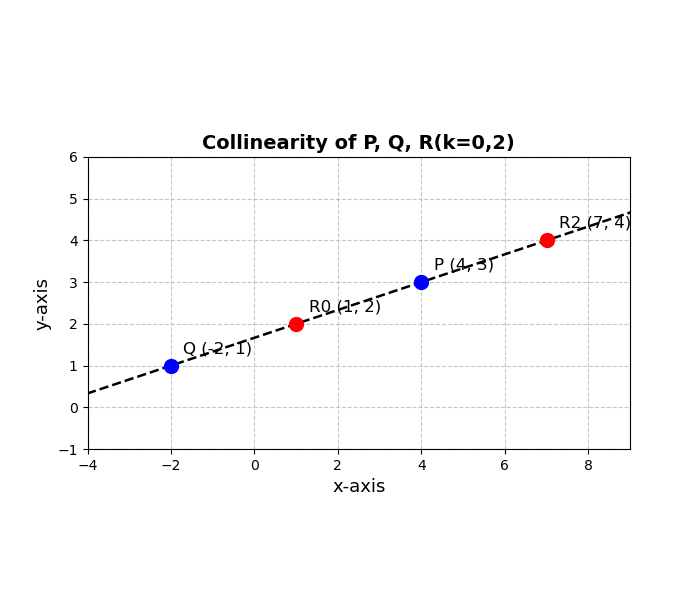
\includegraphics[width=1.0\linewidth]{figs/fig 1.png}
        \caption{Caption}
        \label{fig:placeholder}
    \end{figure}
\end{frame}
\end{document}